\section{条形图}

此前,我们已经学会了如何用SVG绘制简单的矩形、创建比例尺和坐标轴等。现在,我们可以综合运用起来画出一个带有完整信息的条形图。

我们模拟X公司在2011年至2016年期间的股票价格作为数据集,并为它作出条形图实现数据可视化。数据保存在与HTML文件同级目录下,命名为“data.csv”,内容如下:

\begin{minted}[frame=lines,framesep=2mm,baselinestretch=1.2,fontsize=\footnotesize,linenos]{html}
year,value
2011,45
2012,47
2013,52
2014,70
2015,75
2016,78
\end{minted}

接下来,我们将用这份数据创建垂直方向的条形图。

\subsection{建立画布并定义比例尺}

在HTML标签中的body部分建立好SVG画布空间:

\begin{minted}[frame=lines,framesep=2mm,baselinestretch=1.2,fontsize=\footnotesize,linenos]{html}
<body>
    <svg width="600" height="500"></svg>
</body>
\end{minted}

在\verb|<script>|脚本中,为SVG画布定义宽高等,并分别为x轴和y轴创建比例尺,设定了比例尺的值域。

\begin{minted}[frame=lines,framesep=2mm,baselinestretch=1.2,fontsize=\footnotesize,linenos]{html}
<script>
  var svg = d3.select("svg"),
    margin = 200, // 通过margin外边距调整位置
    width = svg.attr("width") - margin,
    height = svg.attr("height") - margin;

  // scaleBand()序数比例尺常用于离散值,如年份
  // padding用于调整条之间的距离
  var xScale = d3.scaleBand().range([0, width]).padding(0.4),
    yScale = d3.scaleLinear().range([height, 0]);
  
  // 创建“组”元素,调整了图表在SVG中的位置
  var g = svg
    .append("g")
    .attr("transform", "translate(" + 100 + "," + 100 + ")");
</script>
\end{minted}

\subsection{加载数据并创建坐标轴}

在上述\verb|<script>|的代码中,继续添加以下这些部分:

\begin{minted}[frame=lines,framesep=2mm,baselinestretch=1.2,fontsize=\footnotesize,linenos]{javascript}
d3.csv("data.csv").then(function (data) {
  xScale.domain(
    data.map(function (d) {
      return d.year;
    })
  );
  yScale.domain([
    0,
    d3.max(data, function (d) {
      return d.value;
    }),
  ]);

  g.append("g")
    .attr("transform", "translate(0," + height + ")")
    .call(d3.axisBottom(xScale));

  g.append("g")
    .call(
      d3
        .axisLeft(yScale)
        .tickFormat(function (d) {
          return "$" + d;
        })
        .ticks(10)
    )
});
\end{minted}

我们来一点点拆解这里新增的代码:

\begin{minted}[frame=lines,framesep=2mm,baselinestretch=1.2,fontsize=\footnotesize,linenos]{javascript}
d3.csv("data.csv").then(function(data) {
  // ...
});
\end{minted}

这一步使用了\verb|d3.csv()|方法加载了数据集\verb|data.csv|。然后,我们可以为x轴和y轴上的比例尺继续添加定义域的范围(在上一步中已经给出了值域)。

\begin{minted}[frame=lines,framesep=2mm,baselinestretch=1.2,fontsize=\footnotesize,linenos]{javascript}
// 使用data.map()映射离散的年份值给x比例尺
xScale.domain(
data.map(function (d) {
  return d.year;
})
);
// 对于y轴,使用d3.max()将定义域设为[0, max]
yScale.domain([
0,
d3.max(data, function (d) {
  return d.value;
}),
]);
\end{minted}

通过创建组(\verb|g|)元素,将x轴添进组元素中,然后我们用\verb|transform|属性来调整其在SVG画布中的位置居底部,并调用了\verb|d3.axisBottom(xScale)|插入了x轴坐标轴。

\begin{minted}[frame=lines,framesep=2mm,baselinestretch=1.2,fontsize=\footnotesize,linenos]{javascript}
g.append("g")
 .attr("transform", "translate(0," + height + ")")
 .call(d3.axisBottom(xScale));
\end{minted}

同样地,我们调用\verb|axisLeft()|在组元素中创建了y轴坐标轴。由于y轴上的元素是股价,我们可以格式化添加\verb|$|的前缀,同时使用了\verb|ticks()|方法来指定y轴大致有多少个区间。

\begin{minted}[frame=lines,framesep=2mm,baselinestretch=1.2,fontsize=\footnotesize,linenos]{javascript}
.tickFormat(function (d) {
  return "$" + d;
})
.ticks(10)
\end{minted}

截止到这里,如\figref{fig:company_axis_xy}所示,我们已经作出了与数据相适应的坐标系。

\begin{figure}[htbp]
    \centering
    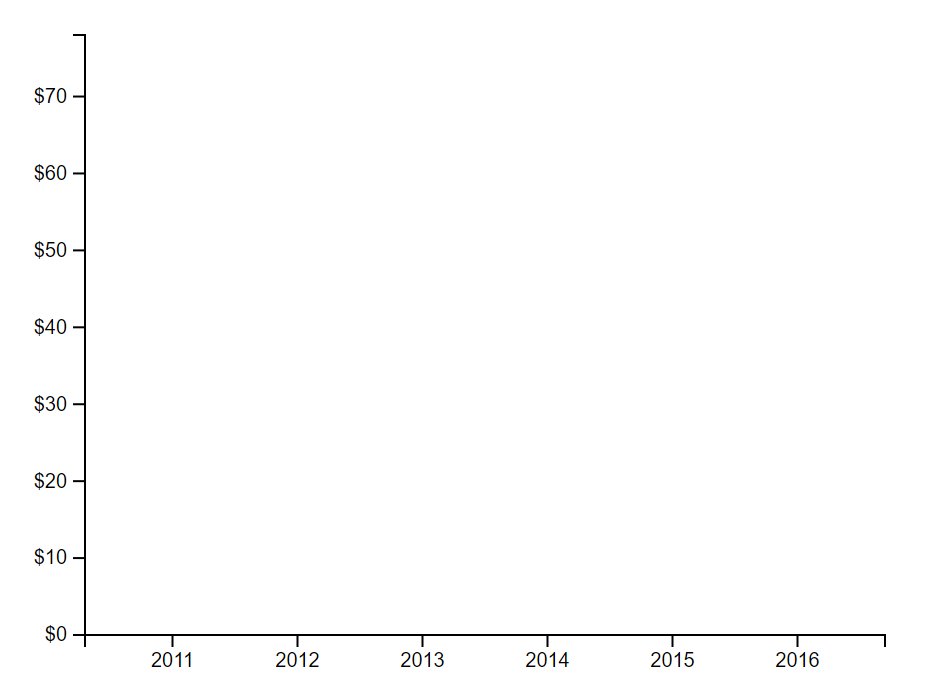
\includegraphics[width=0.6\textwidth]{figure/D3/company_axis_xy.png}
    \caption{\textbf{x、y轴坐标系建立完成}}
    \label{fig:company_axis_xy}
\end{figure}

\subsection{条形绘制}

然后,我们可以在轴上根据数据创建条形。见如下代码(添加在\verb|.csv(){}|函数内部),我在此通过注释方式来讲解。

\begin{minted}[frame=lines,framesep=2mm,baselinestretch=1.2,fontsize=\footnotesize,linenos]{javascript}
g.selectAll(".bar") // 选择所有class为bar的元素
  .data(data)
  .enter()
  .append("rect") // 使用enter()绑定数据
  .attr("class", "bar") // 添加class属性
  .attr("x", function (d) {
    return xScale(d.year);
  }) // x轴坐标为年份
  .attr("y", function (d) {
    return yScale(d.value);
  }) // y轴坐标为股票价格
  .attr("width", xScale.bandwidth())
  // 和x轴下的scaleBand()对应
  .attr("height", function (d) {
    return height - yScale(d.value);
  })
  .attr("fill", "grey");
  // 使用灰色填充,也可以根据.bar写CSS样式来改变颜色
\end{minted}

此时的效果如\figref{fig:company_bar}所示。

\begin{figure}[htbp]
    \centering
    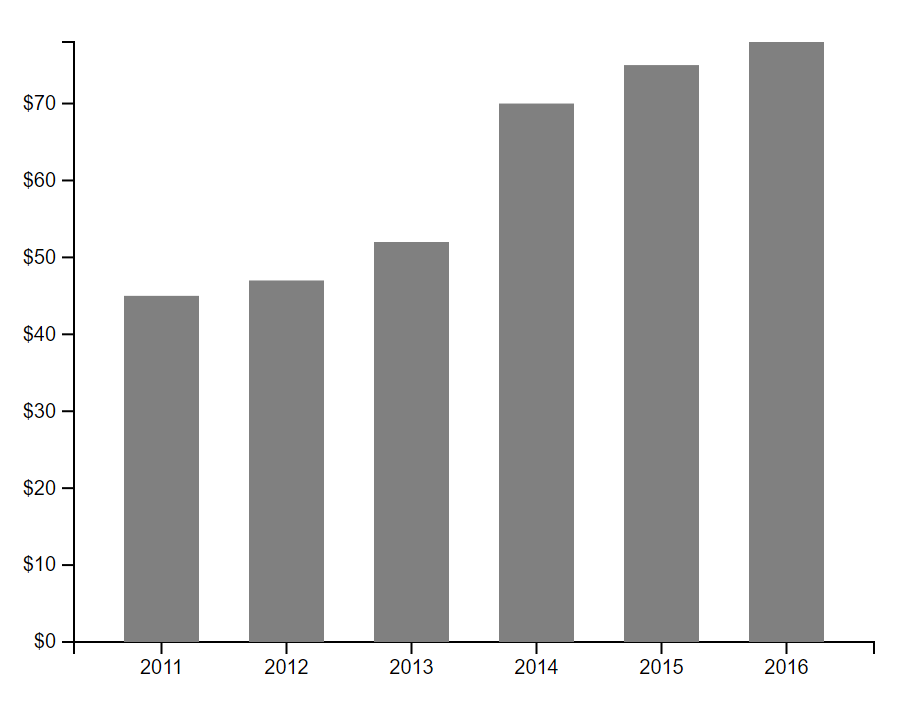
\includegraphics[width=0.6\textwidth]{figure/D3/company_bar.png}
    \caption{\textbf{添加了条形}}
    \label{fig:company_bar}
\end{figure}

\subsection{添加标签}

我们还需要为图表添加标签,如标题、坐标轴上的单位等。使用以下代码添加条形图位于正上方的标题:

\begin{minted}[frame=lines,framesep=2mm,baselinestretch=1.2,fontsize=\footnotesize,linenos]{javascript}
svg
  .append("text")
  .attr("transform", "translate(100,0)")
  .attr("x", 50)
  .attr("y", 50)
  .attr("font-size", "24px")
  .text("X公司股票价格");
\end{minted}

找到此前为x轴和y轴分别使用\verb|axisBottom()|和\verb|axisLeft()|方法创建坐标轴的代码段,修改为:


\begin{minted}[frame=lines,framesep=2mm,baselinestretch=1.2,fontsize=\footnotesize,linenos]{javascript}
g.append("g")
  .attr("transform", "translate(0," + height + ")")
  .call(d3.axisBottom(xScale))
  .append("text")
  .attr("y", height - 250)
  .attr("x", width - 100)
  .attr("text-anchor", "end")
  .attr("stroke", "black")
  .text("年份");

g.append("g")
  .call(
    d3
      .axisLeft(yScale)
      .tickFormat(function (d) {
        return "$" + d;
      })
      .ticks(10)
  )
  .append("text")
  .attr("transform", "rotate(-90)")
  .attr("y", 6)
  .attr("dy", "-5.1em")
  .attr("text-anchor", "end")
  .attr("stroke", "black")
  .text("股价");
\end{minted}

至此,条形图绘制完成,效果如\figref{fig:company_bar_chart_complete}所示。

\begin{figure}[htbp]
    \centering
    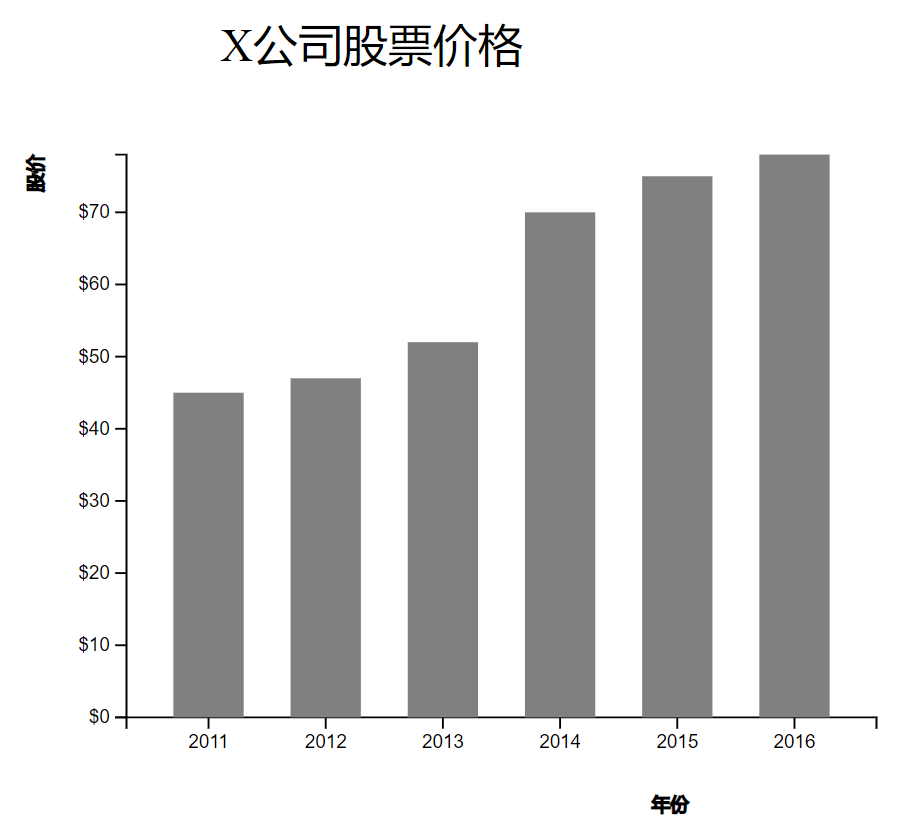
\includegraphics[width=0.6\textwidth]{figure/D3/company_bar_chart_complete.png}
    \caption{\textbf{完整条形图}}
    \label{fig:company_bar_chart_complete}
\end{figure}

以下附上完整代码:

\begin{minted}[frame=lines,framesep=2mm,baselinestretch=1.2,fontsize=\footnotesize,linenos]{html}
<!DOCTYPE html>
<html lang="en">
  <head>
    <meta charset="UTF-8" />
    <meta name="viewport" content="width=device-width, initial-scale=1.0" />
    <title>D3.js</title>
    <!-- 引入D3 -->
    <script src="./js/d3.min.js" charset="utf-8"></script>
  </head>

  <body>
    <svg width="600" height="500"></svg>
  </body>
</html>

<script>
  var svg = d3.select("svg"),
    margin = 200,
    width = svg.attr("width") - margin,
    height = svg.attr("height") - margin;

  var xScale = d3.scaleBand().range([0, width]).padding(0.4),
    yScale = d3.scaleLinear().range([height, 0]);

  var g = svg
    .append("g")
    .attr("transform", "translate(" + 100 + "," + 100 + ")");

  d3.csv("data.csv").then(function (data) {
    xScale.domain(
      data.map(function (d) {
        return d.year;
      })
    );
    yScale.domain([
      0,
      d3.max(data, function (d) {
        return d.value;
      }),
    ]);

    g.append("g")
      .attr("transform", "translate(0," + height + ")")
      .call(d3.axisBottom(xScale))
      .append("text")
      .attr("y", height - 250)
      .attr("x", width - 100)
      .attr("text-anchor", "end")
      .attr("stroke", "black")
      .text("年份");

    g.append("g")
      .call(
        d3
          .axisLeft(yScale)
          .tickFormat(function (d) {
            return "$" + d;
          })
          .ticks(10)
      )
      .append("text")
      .attr("transform", "rotate(-90)")
      .attr("y", 6)
      .attr("dy", "-5.1em")
      .attr("text-anchor", "end")
      .attr("stroke", "black")
      .text("股价");

    g.selectAll(".bar")
      .data(data)
      .enter()
      .append("rect")
      .attr("class", "bar")
      .attr("x", function (d) {
        return xScale(d.year);
      })
      .attr("y", function (d) {
        return yScale(d.value);
      })
      .attr("width", xScale.bandwidth())
      .attr("height", function (d) {
        return height - yScale(d.value);
      })
      .attr("fill", "grey");
  });

  svg
    .append("text")
    .attr("transform", "translate(100,0)")
    .attr("x", 50)
    .attr("y", 50)
    .attr("font-size", "24px")
    .text("X公司股票价格");
</script>
\end{minted}